\chapter{Design}

There are a few core problems to solve.
One is making the participant use the application in the structured way needed to
gather relevant data. The second is to find a way of enableing the developer to integrate
the testing into the application and capture relevant information. The data then needs
to be collected, processed, and presented in a way that makes it easy to spot
problem areas in the interface.

\section{User Facing Design}

On starting the testing, the user is shown a screen explaining how the testing
will work. It outlined the test interface, and what to do if they become stuck.
They are then presented with screen introducing a scenario, and given a task to 
complete, in the same manner as think aloud testing. On
completion of the task, they will be either given a successive task, or a screen
thanking them for participating. Since multiple tasks would usually be presented to the user in a normal testing session, the developer is able to group tasks together to be performed successively. They are also able to control whether a task follows on from the previous one, or whether they all begin from a common screen. This will be useful for most tasks, where, for example, the developer wants the user to start from a specific screen such as the home screen of the application.

\subsection{Early Versions and Gamification}

In an attempt to keep the user being tested engaged, and thus increasing the likelihood they would complete more of the testing, in early iterations the participant would score points by completing tasks. During a task an overlay would show how long the user is taking (\emph{Figure~\ref{fig:initial-overlay}}) and on completion of the task
they would be assigned a number of points relative to how quickly they did it.
Early evaluation of this prototype highlighted a couple of concerns with this approach. Firstly, showing the user how
long they are taking and encouraging them to complete the task as quickly as
possible could cause the participant to focus on the on-screen timer instead of other elements of the interface, resulting in behaviour that did not necessarily match real world usage.
Additionally, the point system did not seem to work as hoped, missing crucial aspects that usually make point systems encouraging.  Since the ``game'' was not really repeatable, and points were not ranked against any other player or used for any other purpose, participants did have an incentive to gather them. 

\begin{figure}[ht!]
  \centering 
  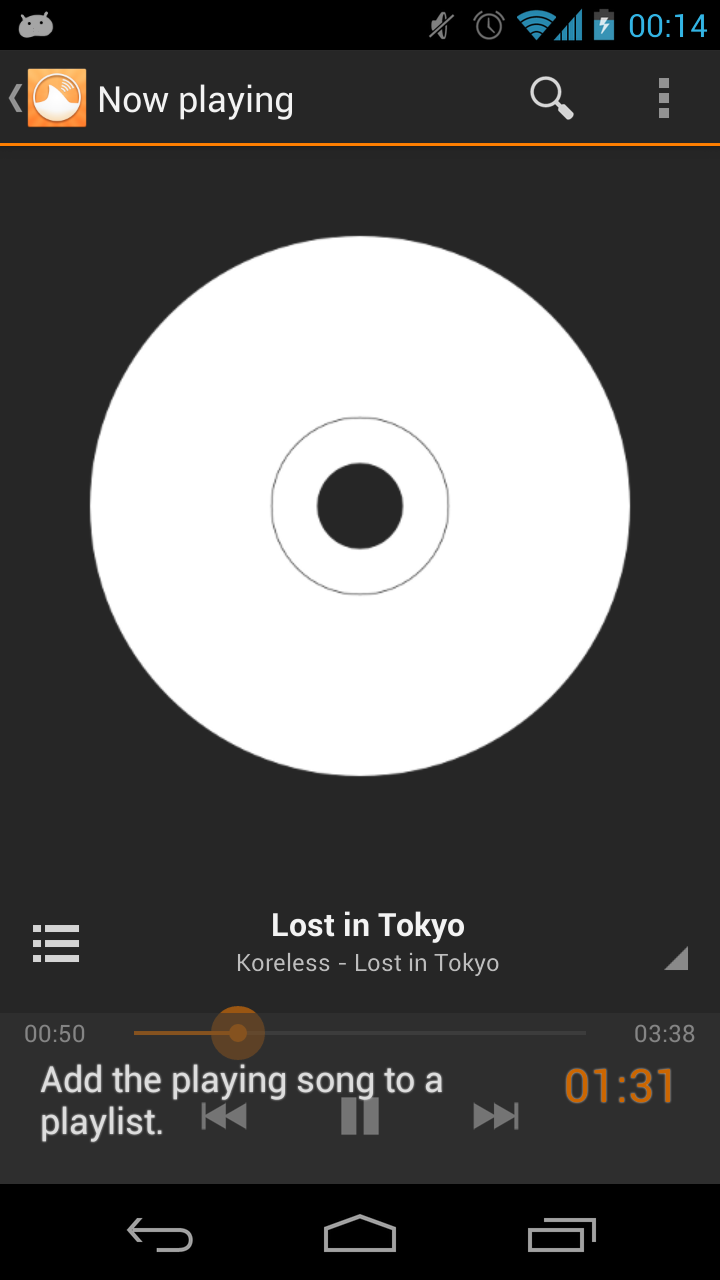
\includegraphics[width=0.5\textwidth]{images/time-taken}
  \caption{The task overlay in early iterations of the project.}
  \label{fig:initial-overlay}
\end{figure}

Due to these issues, the test no longer encourages
the participant to be competitive, removing the timer from the screen during a task. The screen that appears at the beginning of each task now displays
progress that the participant has made through the testing, hopefully encouraging
the user to complete the process. If the developer wishes to provide a reward (such as
unlocking easter eggs or additional features within the app) it would be possible to implement using
the library.

\subsection{In-task UI}

Figure~\ref{fig:initial-overlay} also shows how the early version of the in-task UI was an overlay over the application interface. While this was semi-transparent, it still had a tendency to obscure important controls, making it harder to use the application. This was refined after the initial evaluation so it no longer obscures content while still displaying important information about the task. The final UI can be seen in Figure~\ref{fig:final-task-overlay}. While placing an extra piece of interface at the top of the screen affects the height available to the application, the space taken up is designed to be as small as possible, and android apps must adapt to different screen sizes anyway. This design also facilitates controls being placed in the in-task UI, here used for an ``Abandon'' button.

\begin{figure}[ht]
  \centering
  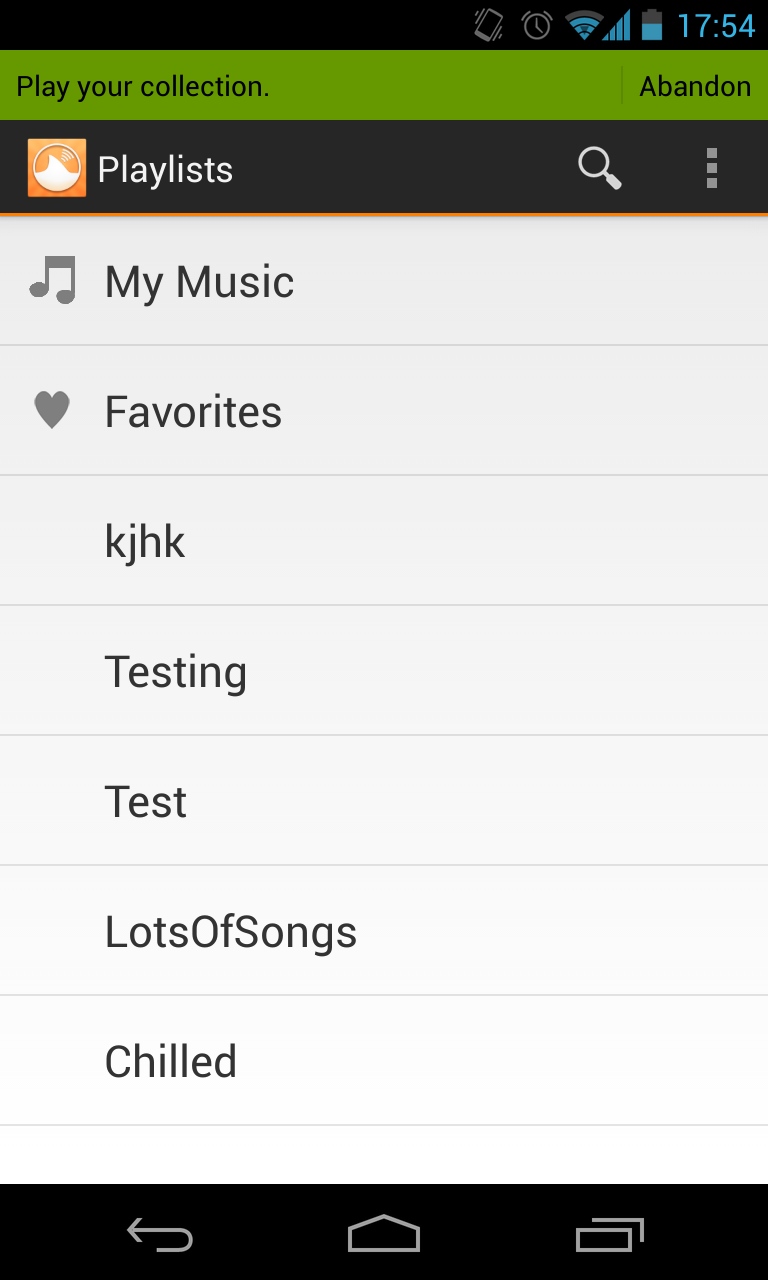
\includegraphics[width=0.5\textwidth]{images/new-in-task}
  \caption{The final iteration of the in-task UI}
  \label{fig:final-task-overlay}
\end{figure}

\subsection{Abandoning Tasks}

It's likely that for some tasks, a participant might get stuck, and not be able
to complete the instruction. In these cases it is important the user does not abandon 
the testing, since the interface could be too unintuitive or confusing. Indeed, this 
is usually the case
where the developer could benefit most from the feedback, so the library must highlight areas
where this scenario happens, and let the testing continue. To
enable this, as part of the overlay that appears while performing a task a
button allows the participant to abandon the current task at any point. This lets them easily continue the testing, and if many people abandon the same task it provides a quick indication of tasks that may be especially difficult to complete.

\section{Developer feedback}
\label{sec:developer-feedback}

To be an effective form of feedback, the system also needs a way for the developer to view the data gathered and identify issues.

There are a few important considerations that were made when designing this interface:

\begin{itemize}
  \item The developer should be able to see as much of the data gathered as possible.
  \item The aggregate performances of many users are far more important than the performance of individual users.
  \item Problem areas within a task should be easy to spot.
  \item Even bigger issues such as tasks that are commonly abandoned should be easy to spot.
\end{itemize}

Some of these criteria are satisfied easily, for example by highlighting tasks with a success rate lower than a certain percentage, but others are harder.

Depending on the data gathered there are a large number of ways of presenting the results to the developer. This project focused on a simple interface which hopes to satisfy the criteria above.

\subsection{Capturing Navigation}

\begin{figure}[h]
 \centering
 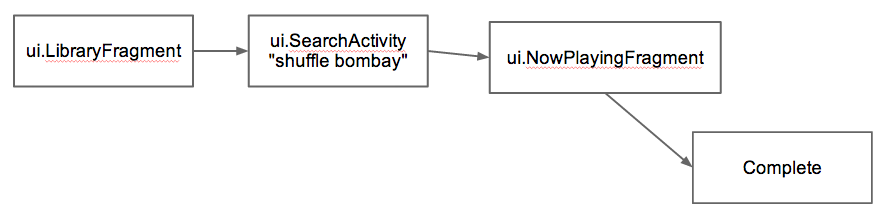
\includegraphics[width=\textwidth]{images/single-path}
 \caption{Mockup of the navigation path of a single user completing a task.}
 \label{fig:task-navigation}
\end{figure}

Each ``run'' through a task can be represented as a sequence of navigation points. Every screen of
an Android app is made up of Activities, or Fragments within an Activity. This provides a starting
point for capturing navigation, so each new Activity created is automatically added as a new navigation point. In addition, 
the developer can choose to include Fragment changes, and any other navigation event that they deem important to 
the data that will be collected. Extra information can be passed along with each point, useful for situations
where the same screen might be used to display different sets of data, for example on a search screen the
developer might want to include the search query used. A simple navigation path is 
shown in Figure~\ref{fig:task-navigation}.

\begin{figure}[h]
 \centering
 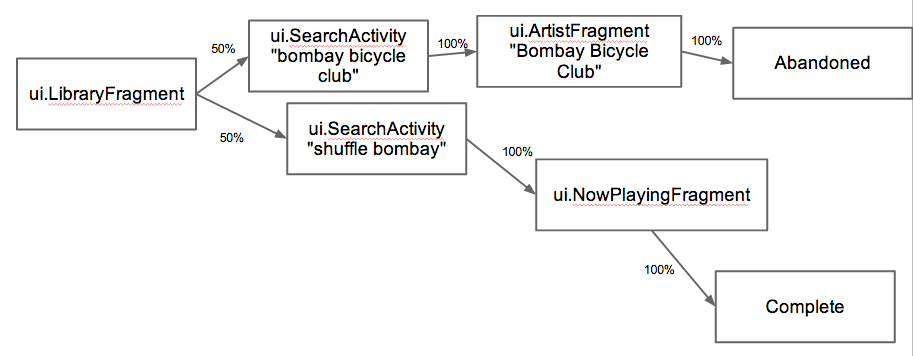
\includegraphics[width=\textwidth]{images/merged-paths}
 \caption{Mockup the navigation path from two users merged together.}
 \label{fig:task-navigation-tree}
\end{figure}

Once the navigation path data has been captured from the completion of a task from a number of participants, the paths are merged to create a navigation graph, as shown in Figure~\ref{fig:task-navigation-tree}. Each path from one node to the next shows the percentage of participants who took that path, and the most
common paths from the start screen to either completing or abandoning the task can be seen.

An issue with this approach immediately showed during early evaluation of the system. When participants were unsure of how to proceed, they would often try many different options, quickly abandoning them and returning to the previous screen when it became clear the action they took was not the correct one.
After a few users doing this the navigation tree became particularly messy and unreadable 
(Figure~\ref{fig:task-navigation-mess}).

\begin{figure}[h]
 \centering
 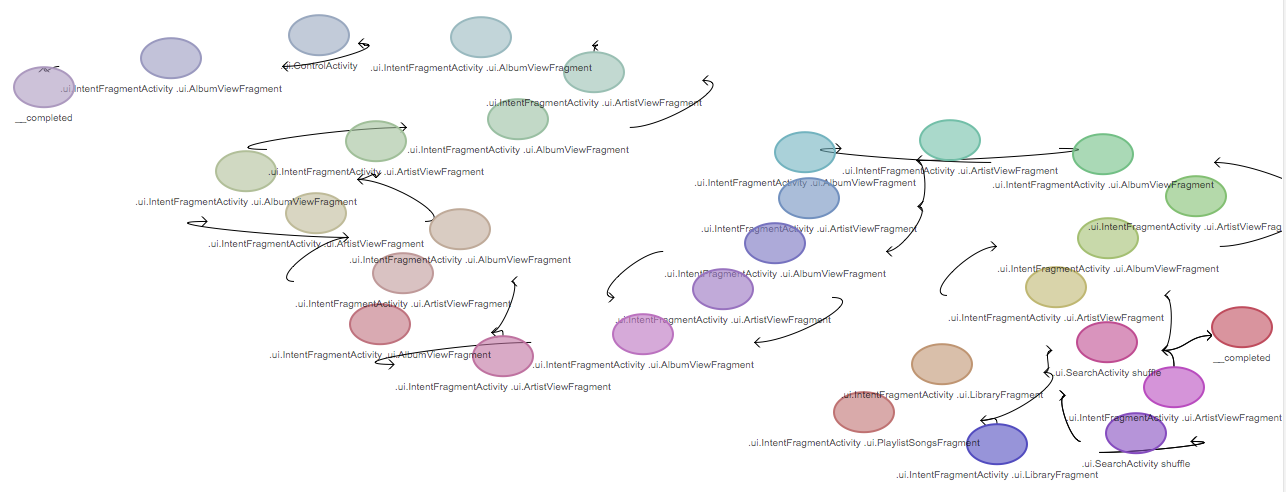
\includegraphics[width=\textwidth]{images/messy-graph}
 \caption{Messy graphs produced when participants backtrack.}
 \label{fig:task-navigation-mess}
\end{figure}

A simple fix was to not include part of the path in the graph when the user immediately returns
to the previous point (Figure~\ref{fig:task-navigation-mess-fixed}). This information is still important to indicate usability problems, so the average number of these ``backtracks'', if any, is shown below each node in the graph indicating potential usability problem areas at a glance.

\begin{figure}[h]
 \centering
 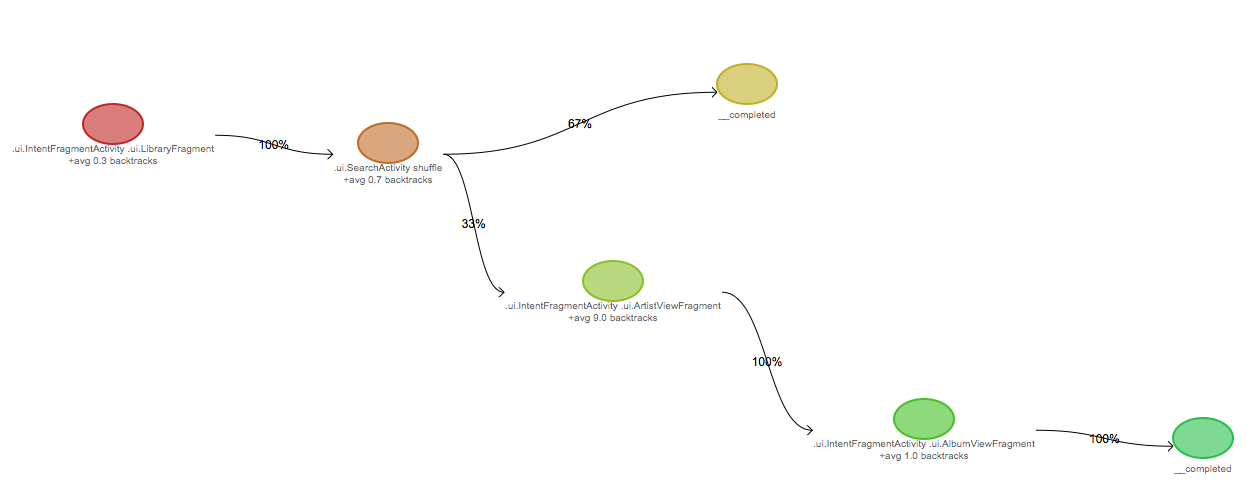
\includegraphics[width=\textwidth]{images/fixed-graph}
 \caption{The same graph after filtering backtracking.}
 \label{fig:task-navigation-mess-fixed}
\end{figure}